% ============================================================
%  CALM-VAD  —  main manuscript
%  Compile:  pdflatex main ; bibtex main ; pdflatex main ; pdflatex main
%  (or just open on Overleaf and hit Recompile)
%
%  Toggle \draftmode below to show/hide the "results pending" banner
%  and the TODO notes. Set to \draftfalse for a clean build.
% ============================================================
\documentclass[conference]{IEEEtran}
\IEEEoverridecommandlockouts

\usepackage{cite}
\usepackage{amsmath,amssymb,amsfonts}
\usepackage{algorithm}
\usepackage{algpseudocode}
\usepackage{graphicx}
\usepackage{booktabs}
\usepackage{multirow}
\usepackage{xcolor}
\usepackage{tikz}
\usetikzlibrary{arrows.meta,positioning,fit,backgrounds,calc}
\usepackage[hidelinks]{hyperref}
\usepackage[capitalize,nameinlink]{cleveref}   % must load after hyperref

% ---- draft switches -------------------------------------------------
\newif\ifdraftmode
\draftmodefalse    % <-- set \draftmodetrue to show the WORKING DRAFT banner again
\ifdraftmode
  \newcommand{\todo}[1]{\textcolor{red!80!black}{\small[\textbf{TODO:} #1]}}
  \newcommand{\pend}[1]{\textcolor{blue!60!black}{#1}}
\else
  \newcommand{\todo}[1]{}
  \newcommand{\pend}[1]{#1}
\fi
\newcommand{\num}[1]{\pend{\texttt{#1}}}   % placeholder for a result number

% ---- notation -----------------------------------------------------
\newcommand{\Rel}{r}                 % reliability
\newcommand{\bel}{\mathrm{Bel}}
\newcommand{\pl}{\mathrm{Pl}}
\newcommand{\me}{m}                  % mass function
\renewcommand{\Theta}{\Omega}       % frame of discernment (Theta is predefined)
\newcommand{\Anom}{\textsf{A}}       % anomaly hypothesis
\newcommand{\Norm}{\textsf{N}}       % normal hypothesis
\newcommand{\faph}{\mathrm{FAPH}}
\newcommand{\ece}{\mathrm{ECE}}
\newcommand{\method}{CALM-VAD}

\begin{document}

\title{\method{}: Calibrated, Auditable, Low-Latency Multi-Cue\\
Video Anomaly Detection for Edge Surveillance}

\author{\IEEEauthorblockN{Faizan Abbas}
\IEEEauthorblockA{Independent Researcher\\
educationpurpose12@outlook.com}}

\maketitle

\ifdraftmode
\begin{center}
\fbox{\parbox{0.94\columnwidth}{\footnotesize\textcolor{red!70!black}{%
\textbf{WORKING DRAFT.} Method, protocol and analysis are complete; the
quantitative tables are populated by the released evaluation harness
(\texttt{calm/harness.py}) and are marked \pend{pending}. Set
\texttt{\textbackslash draftmodefalse} to hide this notice and the TODOs.}}}
\end{center}
\vspace{4pt}
\fi

% ==================================================================
\begin{abstract}
% ----- context
Video anomaly detection (VAD) for public-safety surveillance is increasingly
deployed on resource-constrained edge hardware, yet the systems that run there
share a common back end: a black-box anomaly score followed by a hand-tuned
threshold. Recent audits show that this back end, evaluated by frame-level
AUC, hides catastrophic operating behaviour---tens of thousands of false
alarms per hour at usable recall---and provides operators with neither a
probability they can act on nor an evidence trail they can audit.
% ----- what we do
We present \method{}, a decision layer that replaces the score-and-threshold
back end with four lightweight, well-founded stages: (i) a per-frame
\emph{reliability estimator} for the pose and tracking front end; (ii) a
\emph{reliability-discounted evidence-fusion} layer that combines interpretable
behavioural cues as Dempster--Shafer belief mass, so a degraded skeleton
contributes ignorance rather than a false alarm; (iii) a post-hoc
\emph{calibration map} that turns fused belief into a probability whose value
matches observed incident frequency; and (iv) a \emph{distribution-free
alarm-rate controller} (Learn-then-Test) that admits a threshold only if the
false-alarms-per-hour budget an operator sets is provably met. Each alert is
emitted as an \emph{evidence record}: probability, contributing cues with
weights, sensor reliability, and the budget under which it was raised.
% ----- evaluation
We evaluate on ShanghaiTech, UBnormal, CHAD, Avenue and NWPU-Campus under a
deployment-faithful protocol---event-level $F_1$ at temporal IoU, false
alarms per hour at fixed recall, expected calibration error, cross-dataset
degradation, and CPU latency---rather than frame AUC alone.
% ----- headline
On these five benchmarks \method{}'s calibration stage lowers expected
calibration error by $56$--$95\%$ (e.g.\ $0.41\!\to\!0.02$ on ShanghaiTech,
$0.50\!\to\!0.05$ on UBnormal) with frame AUC left within $0.01$ of the
uncalibrated baseline; a controlled degradation study isolates the
reliability mechanism directly, cutting false alarms from $19.2$ to
$0.0$ per hour at $0.9$ recall when the pose front end is corrupted. With
enough confirmed-normal calibration hours ($0.80\,$h vs.\ $0.07\,$h),
M4 certifies an operator-chosen alarm budget for the first time in this
line of work, and the decision layer adds $0.1$--$1.5$\,ms/frame regardless
of which dataset is running through it. Detection quality is uneven across
benchmarks and we report this honestly: event-level $F_1$ tracks how much of
each benchmark's anomaly taxonomy the five cues actually target, down to two
clean chance-level negative controls (Avenue and NWPU-Campus, whose
anomalies our cues do not model). Code and the evaluation harness are
released.
\end{abstract}

\begin{IEEEkeywords}
video anomaly detection, edge computing, uncertainty calibration, conformal
prediction, Dempster--Shafer fusion, false alarm rate, trustworthy AI
\end{IEEEkeywords}

% ==================================================================
\section{Introduction}
\label{sec:intro}

Automated video anomaly detection is moving from the data centre to the
camera. Public-safety programmes deploy analytics on embedded accelerators
and commodity CPUs at the edge, both to meet latency and bandwidth limits and
to keep raw imagery of uninvolved people from leaving the site
\cite{edgevadsurvey2026,privacyvadsurvey2024}. The AI-video-analytics-for-smart-cities
market is projected to grow from roughly \$8.50\,B in 2025 to \$28.76\,B by 2030,
with public safety its fastest segment and edge deployment a defining trend
\cite{marketaivideo2025}.

Despite this shift, the decision back end of nearly every deployable system is
unchanged from a decade ago: an anomaly model emits a scalar score, and an
operator or integrator sets a threshold on it by hand. Two recent, independent
audits show how poorly this serves deployment. First, frame-level AUC---the
field's dominant metric---does not reflect operating behaviour: at the
threshold that catches 90\% of anomalous frames, off-the-shelf
detectors produce a median of \emph{26{,}000--32{,}000 false alarms per hour}
on a real stream, a volume no human can triage \cite{benchmarkauc2026}.
Second, models that score well on frames flicker between states within an
event, so event-level localisation stays below 10\% at a modest
temporal IoU while frame AUC exceeds 50\% \cite{framestoevents2026}.
Operators respond to this the way the human-factors literature predicts: when
a system's alarms are mostly false, trust and compliance fall to match its
hit rate, and vigilance decays \cite{alertfatigue2025,cctvsemiauto2012,
cctvvigilance2014}.

Three further gaps compound the problem for \emph{pose-based} edge VAD, the
lightweight family that avoids transmitting or modelling raw pixels:

\begin{itemize}
\item \textbf{The score is not a probability.} A reconstruction error or a
hand-weighted sum has no calibrated meaning, so a threshold cannot be chosen
on principled grounds and cannot be compared across sites or time.
\item \textbf{The front end silently corrupts the score.} Occlusion, small
person scale, truncation and identity switches perturb keypoints \emph{before}
any analyzer sees them, and a broken skeleton frequently ``looks anomalous''
\cite{poseChallenges2023,bboxtraj2026}. Reliability is rarely propagated.
\item \textbf{There is no alarm-rate guarantee.} Thresholds are tuned per site
with no statistical control over ``alarms per hour,'' even though
distribution-free machinery for exactly this exists in adjacent fields
\cite{angelopoulos2021ltt,bates2021rcps,seizurercps2023,conformalcps2026}.
\end{itemize}

Finally, regulation is making the missing evidence trail mandatory: the EU AI
Act places biometric and surveillance AI in its high-risk tier, requiring
human oversight, logging and explainability \cite{euaiact2024}.

\medskip\noindent\textbf{Contributions.} We address these gaps with a single
deployable layer and the protocol to evaluate it.

\begin{enumerate}
\item \textbf{Reliability-discounted evidence fusion (M1--M2).} We estimate a
per-frame reliability for the pose/tracking front end from cheap features, and
use it as the discount rate of a Dempster--Shafer combination over
interpretable behavioural cues. A degraded frame moves belief mass to
\emph{ignorance}, not to \emph{anomaly}; inter-cue conflict is retained as an
output. To our knowledge this is the first use of sensor reliability as
belief-mass discounting for multi-cue video anomaly detection.
\item \textbf{Calibrated, budgeted decisions (M3--M4).} We calibrate the fused
belief to an incident probability (verified by expected calibration error) and
apply Learn-then-Test \cite{angelopoulos2021ltt} so an operator names a
false-alarms-per-hour budget $\beta$ and error level $\delta$ and receives a
threshold with $\Pr[\faph \le \beta]\ge 1-\delta$. This is, to our knowledge,
the first VAD system admitted under a distribution-free alarm-rate guarantee.
\item \textbf{The evidence record.} Every alert is a structured record---
probability, per-cue belief and discount, conflict, reliability, and the
admitting budget---directly usable as the audit artifact that oversight
regimes require \cite{euaiact2024}.
\item \textbf{A deployment-faithful evaluation harness.} We release a
reproducible protocol combining event-level $F_1$ at temporal IoU, false
alarms per hour at fixed recall, calibration error, cross-dataset degradation
and CPU latency, and use it to study \method{} against weighted-sum, logistic
and gradient-boosted baselines with full ablations.
\end{enumerate}

\method{} is built on an existing open pose-VAD pipeline (17-keypoint skeletons
\cite{ultralytics2023} + ByteTrack \cite{bytetrack2022} + five behavioural
cues: fall, fight, loitering, abandoned object, crowd). The perception front
end and the cues are unchanged; the contribution is the decision layer and the
evaluation around it.

% ==================================================================
\section{Related Work}

\subsection{Pose- and skeleton-based VAD}
Skeleton input discards appearance and background, which lowers compute and
improves privacy; recent methods model normal skeleton dynamics with
normalizing flows \cite{stgnf2023}, diffusion \cite{graphjigsaw2024},
autoregressive density \cite{seeker2025}, or cross-domain semantic cues
\cite{actionhints2025}. These produce a single unsupervised score, are
evaluated by frame AUC, and---as \cite{poseChallenges2023,bboxtraj2026}
document---degrade when pose estimation fails. The reliability-aware prototype
calibration method \cite{reliabilityproto2026} is the closest prior work: for
a single frozen pose-flow backbone, it adds a nearest-prototype deviation
term to the flow score, gated by keypoint confidence, and reports frame
AUROC gains averaging 2.03 points across eight backbone-dataset pairs (no
event-level, false-alarm, or calibration-error metric is reported).
\method{} differs in three ways: reliability enters as \emph{evidence
discounting across a fused, heterogeneous cue set} with an explicit conflict
term, not a single-backbone score correction; the output is a post-hoc
\emph{probability} with a distribution-free alarm-budget guarantee, not a
rank-only AUROC correction; and it is evaluated for alarm load, event
localisation and calibration error, not frame AUC alone.

\subsection{Lightweight and edge VAD}
Edge-oriented work targets latency and memory, often with a cheap first stage
and a heavier verifier \cite{edgevadsurvey2026,nsvad2024}. The system nearest
to ours in stack \cite{yoloposeclip2026} pairs YOLO-pose with CLIP
prompt-similarity at 51\,fps on a GPU, reporting frame AUROC only, with no
fusion, calibration, guarantee or false-alarm analysis. We share the front end
and add the decision layer it lacks, on CPU.

\subsection{Explainable VAD}
Vision-language methods emit natural-language rationales \cite{vera2025}; a
transformer with SHAP attributions produces an interpretable ``suspiciousness''
regressor \cite{deepusevision2025}. Neither reports calibration, a conformal
guarantee, or false alarms per hour, and both require a GPU;
\cite{deepusevision2025} is single-frame and uses affect cues that
action-only systems avoid on reliability grounds. \method{}'s explanation is
the belief decomposition itself---auditable and free---rather than a generated
sentence or a post-hoc attribution.

\subsection{Calibration and distribution-free risk control}
Post-hoc calibration (Platt \cite{platt1999}, isotonic
\cite{zadrozny2002isotonic}, temperature \cite{guo2017calibration}) and ECE
\cite{naeini2015ece} are standard in classification but rarely reported for
VAD \cite{benchmarkauc2026}. Learn-then-Test \cite{angelopoulos2021ltt} and
risk-controlling prediction sets \cite{bates2021rcps} build on conformal
prediction's distribution-free coverage guarantees \cite{vovk2005algorithmic}
to give model-agnostic, finite-sample control of an arbitrary risk; they have
been applied to seizure
false-alarm control \cite{seizurercps2023} and industrial CPS
\cite{conformalcps2026}, but not, to our knowledge, to video surveillance
anomaly detection. We instantiate them with ``false alarms per hour of normal
stream'' as the controlled risk.

\subsection{Evidence fusion}
Dempster--Shafer theory \cite{shafer1976,smets1994tbm} is a mature tool for
fusing uncertain, conflicting sources and is valued for interpretability; it
is standard in intrusion detection \cite{dsids2005} and multi-sensor systems.
Its use here---discount rates tied to a learned pose/tracking reliability,
combined with a calibration map and a conformal alarm budget---is, to our
knowledge, new for real-time edge pose VAD.

\Cref{tab:positioning} summarises how \method{} positions against the systems
and audits discussed in this section, across the capabilities that matter for
deployment.

% Capability matrix. cmark / pmark / xmark defined here for portability.
\providecommand{\cmark}{\textbf{\textcolor{green!45!black}{\checkmark}}}
\providecommand{\pmark}{\textcolor{orange!80!black}{$\sim$}}
\providecommand{\xmark}{\textcolor{red!60!black}{$\times$}}
\begin{table}[t]
\centering
\caption{Capability coverage. \cmark~delivered, \pmark~partial/adjacent,
\xmark~absent. No prior row carries \cmark{} across the last four columns
together.}
\label{tab:positioning}
\setlength{\tabcolsep}{3pt}
\renewcommand{\arraystretch}{1.15}
\footnotesize
\begin{tabular}{@{}lcccccc@{}}
\toprule
System / line of work & \rotatebox{90}{interp.\ fusion} & \rotatebox{90}{calib.\ prob.}
 & \rotatebox{90}{reliab.$\to$score} & \rotatebox{90}{alarm guarantee}
 & \rotatebox{90}{deploy.\ protocol} & \rotatebox{90}{edge/CPU} \\
\midrule
Base pipeline (weighted sum)        & \pmark & \xmark & \xmark & \xmark & \xmark & \cmark \\
Pose density \cite{stgnf2023,graphjigsaw2024} & \xmark & \xmark & \xmark & \xmark & \xmark & \pmark \\
YOLO-pose + CLIP \cite{yoloposeclip2026}      & \xmark & \xmark & \xmark & \xmark & \xmark & \pmark \\
VLM-explainable \cite{vera2025}               & \pmark & \xmark & \xmark & \xmark & \xmark & \xmark \\
Fusion + SHAP \cite{deepusevision2025}        & \cmark & \xmark & \xmark & \xmark & \xmark & \xmark \\
Reliab.\ prototype \cite{reliabilityproto2026}& \xmark & \pmark & \cmark & \xmark & \xmark & \pmark \\
``AUC $\neq$ reliability'' \cite{benchmarkauc2026} & --- & \pmark & \xmark & \xmark & \cmark & --- \\
Learn-then-Test \cite{angelopoulos2021ltt}    & --- & \pmark & \xmark & \cmark & \xmark & --- \\
\textbf{CALM-VAD (ours)} & \cmark & \cmark & \cmark & \cmark & \cmark & \cmark \\
\bottomrule
\end{tabular}
\end{table}


% ==================================================================
\section{Problem Formulation}
\label{sec:problem}

A camera produces frames at rate $\phi$ (fps). A perception front end yields,
per frame $t$, a set of tracked persons with 17-keypoint skeletons and a set
of tracked objects. A bank of $C$ behavioural cues maps this to a
\emph{strength} vector $\mathbf{s}_t\in[0,1]^C$, where $s_{t,c}$ measures how
far cue $c$ is past its confirmation condition ($0$: not firing; $1$: firmly
confirmed). Ground truth is a set of anomaly \emph{events}
$\mathcal{E}=\{(a_k,b_k)\}$, each a maximal interval of frames.

\paragraph{Detection targets}
Given a per-frame score $p_t$ and threshold $\tau$, predicted events are the
maximal runs of $\{t: p_t\ge\tau\}$ after debouncing gaps shorter than
$g$ seconds (\texttt{min\_gap\_s}, default $3.0$) and dropping any resulting
run shorter than a minimum duration $\ell$ seconds (\texttt{min\_len\_s},
default $0.3$). For a temporal-IoU threshold $\theta$, event $F_1(\theta)$ uses
one-to-one greedy matching of predicted to ground-truth events with
$\mathrm{tIoU}\ge\theta$; we report $\bar F_1=\operatorname{mean}_\theta
F_1(\theta)$ over $\theta\in\{0.2,0.3,0.4,0.5\}$ \cite{framestoevents2026}.

\paragraph{Alarm load}
Let $T_{\text{n}}$ be the number of hours of \emph{non-anomalous} stream, and
let a \emph{false-alarm event} be a predicted event overlapping no
ground-truth event. The false-alarms-per-hour at threshold $\tau$ is
\begin{equation}
\faph(\tau)=\frac{\#\{\text{false-alarm events}\}}{T_{\text{n}}}.
\end{equation}
We report $\faph$ at the least $\tau$ whose event recall meets a target
$\rho\in\{0.7,0.8,0.9\}$, and at the operator budget (below).

\paragraph{Calibration}
With per-window incident labels $y_t\in\{0,1\}$, the (binned) expected
calibration error is
\begin{equation}
\ece=\sum_{b=1}^{B}\frac{|I_b|}{n}\,\bigl|\operatorname{acc}(I_b)-\operatorname{conf}(I_b)\bigr|,
\end{equation}
with $I_b$ the windows whose $p_t$ falls in bin $b$; we also report the
equal-mass (adaptive) variant and the Brier score.

\paragraph{Operator budget}
The operator specifies a tolerated rate $\beta$ (false alarms per hour) and an
error level $\delta$. A controller is \emph{valid} if the threshold $\tau$ it
returns satisfies $\Pr[\faph(\tau)\le\beta]\ge 1-\delta$, the probability over
the calibration sample.

% ==================================================================
\section{Method: \method{}}
\label{sec:method}

\subsection{Overview}
\Cref{fig:arch} contrasts the baseline back end with \method{}. The front end
(pose, tracking) and the cue bank are untouched. \method{} adds: M1, a
reliability estimate $\Rel_t$ for the frame's skeletons and tracks; M2, a
reliability-discounted Dempster--Shafer fusion of the cues into a belief
$\bel_t(\Anom)$ and a conflict $K_t$; M3, a calibration map
$g:\bel\mapsto p$; and M4, a Learn-then-Test choice of $\tau$ meeting the
operator budget. The alert is the evidence record of
\cref{sec:record}.

\begin{figure}[t]
\centering
% Baseline vs CALM-VAD back end. Included by main.tex (needs tikz + libraries
% arrows.meta, positioning, fit, backgrounds, calc). Draws inside one column.
\resizebox{\columnwidth}{!}{%
\begin{tikzpicture}[
  font=\footnotesize,
  box/.style={draw, rounded corners=1pt, minimum height=8mm, minimum width=15mm,
              align=center, inner sep=2pt},
  add/.style={box, fill=black!7, thick},
  fl/.style={-{Stealth[length=1.6mm]}, shorten >=1pt, shorten <=1pt},
  node distance=4mm and 6mm,
]

% ---------- baseline row ----------
\node[box] (b1) {pose\\+ track};
\node[box, right=of b1] (b2) {5 cue\\analyzers};
\node[box, right=of b2] (b3) {weighted\\sum};
\node[box, right=of b3] (b4) {hand\\threshold};
\node[box, right=of b4] (b5) {alert};
\foreach \a/\b in {b1/b2,b2/b3,b3/b4,b4/b5} \draw[fl] (\a) -- (\b);
\node[left=3mm of b1, align=right, text=black!55] {\scriptsize BASELINE};
\node[below=1mm of b3, text=red!60!black] {\scriptsize uncalibrated \# \ \ no guarantee \ \ no trail};

% ---------- CALM-VAD row ----------
\node[box, below=15mm of b1] (c1) {pose\\+ track};
\node[box, right=of c1] (c2) {5 cue\\analyzers};
\node[add, right=9mm of c2] (m2) {\textbf{M2}\\evidence\\fusion};
\node[add, right=of m2] (m3) {\textbf{M3}\\calibrate\\$\to p$};
\node[add, right=of m3] (m4) {\textbf{M4}\\LTT gate\\$\beta$/hr};
\node[box, right=of m4] (c5) {alert +\\record};
\node[add, below=6mm of m2] (m1) {\textbf{M1}\\reliability $r$};

\foreach \a/\b in {c1/c2,c2/m2,m2/m3,m3/m4,m4/c5} \draw[fl] (\a) -- (\b);
\draw[fl] (m1) -- (m2);
\draw[fl] (c2.south) |- (m1.west);
\node[left=3mm of c1, align=right, text=black!55] {\scriptsize \textbf{CALM-VAD}};

% brace-ish label under the added chain
\begin{scope}[on background layer]
  \node[draw=black!25, rounded corners=2pt, fill=black!3,
        fit=(m1)(m2)(m3)(m4), inner sep=3pt] {};
\end{scope}
\node[below=1mm of m1, text=black!55] {\scriptsize added decision layer};

\end{tikzpicture}}

\caption{Baseline score-and-threshold back end (top) vs.\ \method{} (bottom).
The perception front end and the five cues are unchanged; the contribution is
the shaded chain M1--M4 and the evidence record.}
\label{fig:arch}
\end{figure}

\subsection{M1: Front-end reliability}
\label{sec:m1}
For a tracked person $i$ at frame $t$ we form a feature vector
$\mathbf{x}_{t,i}\in[0,1]^7$ from quantities already in the pipeline: mean
keypoint confidence, torso-keypoint confidence, fraction of visible joints,
normalised person scale (pixel height / frame height), an un-truncation ratio
(visible bbox area / bbox area), track stability (a ramp that resets on an
identity switch), and temporal smoothness ($1-$ torso-normalised keypoint
jitter). The reliability is
\begin{equation}
\Rel_{t,i}=\operatorname{clip}\!\bigl(\sigma(\mathbf{w}^\top\mathbf{x}_{t,i}+w_0),\;\Rel_{\min},\Rel_{\max}\bigr),
\end{equation}
with $\sigma$ the logistic function. In the \emph{heuristic} mode $\mathbf{w}$
is a fixed convex combination (no $\sigma$); in the \emph{fitted} mode
$(\mathbf{w},w_0)$ is a logistic regression trained against a proxy quality
label---temporal IoU of the predicted skeleton against a reference, or
agreement between the pose cue and a bounding-box-trajectory cue
\cite{bboxtraj2026}. The per-frame reliability driving M2 is the mean of
$\Rel_{t,i}$ over the persons who contribute to an active cue (or $1$ when no
skeleton is involved, e.g.\ a crowd-count frame).

\subsection{M2: Reliability-discounted evidence fusion}
\label{sec:m2}
The frame of discernment is $\Theta=\{\Anom,\Norm\}$; a mass function assigns
belief to $\{\Anom\}$, $\{\Norm\}$ and $\Theta$ (ignorance), summing to $1$.
Cue $c$ with strength $s$ yields
\begin{align}
\me_c(\{\Anom\}) &= s, \\
\me_c(\{\Norm\}) &= (1-s)\,\rho_c, \\
\me_c(\Theta) &= 1-\me_c(\{\Anom\})-\me_c(\{\Norm\}),
\end{align}
where $\rho_c\in[0,1]$ encodes how strongly a \emph{silent} cue implies
normality (small for loitering, larger for a held fall). We then apply
Shafer discounting twice---once by the cue-type reliability $\Rel_c$
(configured; a held fall is stronger evidence than a crowd count) and once by
the per-frame front-end reliability $\Rel_t$ from M1:
\begin{equation}
\me'(X)=\Rel\,\me(X)\ \ (X\neq\Theta),\qquad
\me'(\Theta)=\Rel\,\me(\Theta)+(1-\Rel).
\end{equation}
Discounted cues are combined with a standing normal prior by Dempster's rule;
for two masses over $\Theta$,
\begin{equation}
(\me_1\!\oplus\!\me_2)(X)=\frac{1}{1-K}\sum_{Y\cap Z=X}\me_1(Y)\,\me_2(Z),
\end{equation}
\begin{equation}
K=\sum_{Y\cap Z=\varnothing}\me_1(Y)\,\me_2(Z).
\end{equation}
The fusion outputs $\bel(\Anom)=\me(\{\Anom\})$, the plausibility
$\pl(\Anom)=\me(\{\Anom\})+\me(\Theta)$, and the accumulated conflict $K_t$.
A large $K_t$ means the cues disagree and is surfaced to the operator even
when $\bel(\Anom)$ is mid-range. Every term above is inspectable, so an alert
decomposes into per-cue mass and the discount applied.

\subsection{M3: Calibration}
\label{sec:m3}
$\bel_t(\Anom)$ is monotone in ``how anomalous'' but is not a frequency. On a
held-out calibration split with labels $y_t$ we fit a monotone map
$g:\!\bel\mapsto p$ (isotonic regression by default \cite{zadrozny2002isotonic};
Platt \cite{platt1999} or temperature \cite{guo2017calibration} for small
splits), freeze it, and report $\ece$, adaptive-$\ece$ and Brier on the test
split, before and after $g$.

\subsection{M4: Distribution-free alarm-rate control}
\label{sec:m4}
We control $\faph$ with Learn-then-Test \cite{angelopoulos2021ltt} over a
descending grid of thresholds $\tau_1>\dots>\tau_m$. On a calibration stream
of $T$ confirmed-normal hours, let $N(\tau)$ be the debounced false-alarm
event count at $\tau$. Modelling rare independent alarms as Poisson, the exact
upper $1-\delta$ confidence bound on the rate is
\begin{equation}
\widehat{\faph}_{\text{hi}}(\tau)=\frac{1}{2T}\,\chi^2_{1-\delta}\!\bigl(2(N(\tau)+1)\bigr).
\end{equation}
Because the nulls $\{\faph(\tau_j)>\beta\}$ are nested (if it fails at $\tau_j$
it fails for every smaller threshold), fixed-sequence testing is valid without
multiplicity correction: walk $\tau_1\!\to\!\tau_m$, admit while
$\widehat{\faph}_{\text{hi}}(\tau_j)\le\beta$, and stop \emph{admitting}
further thresholds at the first violation (\cref{alg:ltt}). Deploy the most sensitive admitted threshold; if none is
admitted, return the most conservative $\tau_1$ and report that the budget
could not be certified on the available normal hours.

\begin{algorithm}[t]
\caption{M4 --- alarm-rate control (Learn-then-Test)}
\label{alg:ltt}
\begin{algorithmic}[1]
\Require calibrated scores $p^{\text{n}}$ on $T$ normal hours; budget $\beta$;
level $\delta$; grid $\tau_1>\dots>\tau_m$
\State $\mathcal{A}\gets\varnothing$
\For{$j=1,\dots,m$}
  \State $N\gets\textsc{DebouncedEventCount}(p^{\text{n}},\tau_j)$
  \State $u\gets \tfrac{1}{2T}\,\chi^2_{1-\delta}(2(N{+}1))$
  \If{$u\le\beta$}
    \State $\mathcal{A}\gets\mathcal{A}\cup\{\tau_j\}$
  \Else
    \State \textbf{stop admitting} \Comment{fixed-sequence stop: no later
      $\tau_j$ joins $\mathcal{A}$; the released implementation keeps
      walking the grid only to log a diagnostic row per $\tau_j$}
  \EndIf
\EndFor
\State \Return $\min\mathcal{A}$ if $\mathcal{A}\neq\varnothing$ else $\tau_1$
\end{algorithmic}
\end{algorithm}

\subsection{The evidence record}
\label{sec:record}
An alert is a structured record: timestamp; calibrated $p$; decision
$p\!\ge\!\tau$; threshold $\tau$ and the $(\beta,\delta)$ it was admitted
under; $\bel(\Anom)$, $\pl(\Anom)$, conflict $K$; front-end reliability
$\Rel$; and the list of contributing cues, each with its (discounted) mass and
strength. It is logged alongside the frame and is the artifact an oversight
process inspects \cite{euaiact2024}.

% ==================================================================
\section{Experimental Setup}
\label{sec:setup}

\Cref{fig:protocol} lays out the five evaluation axes used through the rest
of this section and where each attaches to the path from per-frame score to
operator action.

\begin{figure}[t]
\centering
% The five evaluation axes and where each attaches to the score -> action path.
\resizebox{\columnwidth}{!}{%
\begin{tikzpicture}[
  font=\footnotesize,
  stage/.style={draw, rounded corners=1pt, minimum height=8mm, minimum width=17mm, align=center},
  axis/.style={draw, dashed, rounded corners=1pt, fill=black!4, align=center,
               minimum height=7mm, inner sep=2pt, text=black!70},
  fl/.style={-{Stealth[length=1.6mm]}},
  node distance=8mm,
]
\node[stage] (s1) {per-frame\\score $p_t$};
\node[stage, right=of s1] (s2) {debounced\\event};
\node[stage, right=of s2] (s3) {threshold\\$\tau$ (M4)};
\node[stage, right=of s3] (s4) {operator};
\foreach \a/\b in {s1/s2,s2/s3,s3/s4} \draw[fl] (\a) -- (\b);

\node[axis, above=6mm of s1] (a1) {calibration:\\ECE, Brier};
\node[axis, above=6mm of s2] (a2) {detection:\\event $F_1$@tIoU};
\node[axis, above=6mm of s3] (a3) {alarm load:\\FAPH @ recall / $\beta$};
\node[axis, below=6mm of s2] (a4) {cost:\\ms/frame on CPU};
\node[axis, below=6mm of s3] (a5) {generalisation:\\train $A$, test $B$};

\foreach \a/\s in {a1/s1,a2/s2,a3/s3} \draw[fl, black!45] (\a) -- (\s);
\foreach \a/\s in {a4/s2,a5/s3} \draw[fl, black!45] (\a) -- (\s);
\end{tikzpicture}}

\caption{The five evaluation axes and where each is measured on the path from
per-frame score to operator action.}
\label{fig:protocol}
\end{figure}

\paragraph{Datasets}
All five are complete: ShanghaiTech \cite{shanghaitech2017} (official test
split, 107 clips) and UBnormal \cite{ubnormal2022} (official test split, 211
clips; one -- a smoke-scenario clip with zero detected pose frames -- is
dropped by the harness before scoring, leaving 210), CHAD \cite{chad2023}
(official \texttt{test\_split\_1}, 134 clips), Avenue \cite{avenue2013} (21
test clips), and NWPU-Campus \cite{nwpu2023} (official test split, 242
clips). NWPU-Campus was the hardest to obtain: its release ships only raw
video (76.6\,GB, split across a 106-volume \texttt{.7z}
archive with no per-clip boundaries -- no partial download is possible), and
the only other lead we found, the original authors' own tracking bundle, ships
bounding boxes with no keypoints, insufficient for M1 or FALL/FIGHT. A real
result needed the GPU pose-extraction pass over the full video release we had
flagged as future work; we since ran it (Colab, T4, in batches to fit a
64\,GB disk budget) and it is included below.

\paragraph{Pose extraction}
No video or GPU step was needed for three of the five: ShanghaiTech and
UBnormal poses come from the STG-NF release \cite{stgnf2023} (AlphaPose,
person-major per-clip JSON); CHAD ships 17-keypoint COCO pose and bounding-box
annotations natively (per-frame pickles) from its own release
\cite{chad2023}. Avenue and NWPU-Campus have no pose release, so we extracted
both ourselves with YOLO11n-pose \cite{ultralytics2023} + ByteTrack
\cite{bytetrack2022}: Avenue on CPU (video via the direct, checksummed URLs
published in the \texttt{anomalib} library's dataset module), NWPU-Campus on
a Colab T4 GPU (video via the official release, one archive read directly
from Drive with no local copy of the 76.6\,GB archive, to fit the runtime's
disk budget). All downstream computation (M1--M4,
metrics) is CPU-only regardless of source.

\paragraph{Splits}
Each dataset is divided into calibration (M3 fit; the normal portion drives
M4) and test. Cross-dataset runs fit M3/M4 on dataset $A$ and evaluate on $B$.
ShanghaiTech needed a fix worth documenting rather than hiding: our
pose-conversion file stored 106 of its 107 official clips twice
(byte-identical duplicate JSON records once each frame's person-list is
sorted by track id -- the two copies differed only in per-frame detection
order), so the harness used to ingest 213 raw records; the calibration
carve-out deduplicated by clip name when drawing a 36-clip calibration split,
then removed every raw record sharing one of those 36 names from the test
pool, leaving ``141 test clips'' that were actually 141 raw records covering
only 71 unique clips (most duplicated once, so most test-set frames were
counted twice in the pooled metrics). We have since corrected this: the
pose-conversion file was deduplicated to its true 107 unique clips (one copy
kept per clip, verified byte-identical after the track-id sort before either
copy was dropped), and every ShanghaiTech-derived result in this paper --
in-domain, cross-benchmark, ablations and cross-dataset -- was regenerated
from that corrected file. The harness now carves a 35-clip calibration split
from the 107 unique clips, leaving 72 test clips, each counted once.

\paragraph{Baselines}
Implemented and run on every dataset: \textbf{B0} the weighted-sum fusion of
the base pipeline (calibrated identically to \method{} for a fair ECE
comparison; implemented in \texttt{calm/harness.py} as
\texttt{\_weighted\_sum\_scores()}, separate from SENTRIX's live-deployment
\texttt{ThreatFusion} module in \texttt{src/fusion.py}, never imported by
\texttt{calm/}); \textbf{B1} logistic regression on the cue-strength vector;
\textbf{B2} gradient-boosted trees on the same; \textbf{B4} the single
strongest cue with no fusion at all (\S\ref{sec:ablations}).
\textbf{B3} -- a published pose-density score such as STG-NF's own trained
normalizing-flow model \cite{stgnf2023} -- is deliberately left out: a fair
run would mean cloning and training that method's full codebase rather than
consuming a released score file (none is published), which is a different
scope of work from evaluating our own back end, so we cite its numbers
rather than reproduce them and do not claim a head-to-head comparison.

\paragraph{Ablations}
$-$M1 (no reliability discount) is run as a separate stream on every dataset.
M3's effect is measured directly as raw-vs-calibrated $\ece$ within the same
run; M4's effect is the certified/not-certified outcome at each budget
(\S\ref{sec:m4} results). Two further sweeps are run on all five benchmarks
and reported in \S\ref{sec:ablations}: a \emph{fusion-variant} sweep
(Dempster's rule, the \method{} default, vs.\ noisy-OR combination, vs.\ B4's
no-fusion baseline, holding M1 discounting and M3 calibration fixed) and a
\emph{calibration-variant} sweep (isotonic, the default, vs.\ Platt vs.\
temperature scaling, holding the fused belief fixed).

\paragraph{Metrics}
As in \cref{sec:problem}: frame AUC, $\bar F_1$ and $F_1(\theta)$; $\faph$ at
$\rho\in\{0.7,0.8,0.9\}$ and at $\beta\in\{2,5,10\}$; $\ece$, adaptive-$\ece$,
Brier; cross-dataset absolute drop; decision-layer ms/frame and end-to-end fps.

\paragraph{Hardware}
Decision layer, metrics, and the Avenue pose extraction all ran on the same
commodity laptop CPU: an Intel Core i5-6300U (2 cores / 4 threads,
2.4\,GHz), 12\,GB RAM, Windows 10, Python 3.12. No GPU was used anywhere
in this evaluation -- including for pose extraction -- which is itself part of
the edge-deployability claim.

% ==================================================================
\section{Results}
\label{sec:results}

\ifdraftmode
\noindent\textcolor{red!70!black}{\small The tables below give the exact rows
the released harness (\texttt{python -m calm.harness}) produces; cells are
\pend{pending} the experimental campaign. The analysis text states the
hypothesis each table tests.}
\medskip
\fi

\subsection{Detection and alarm load}
% Populated from results/calm_report_shanghaitech.json (real STG-NF ShanghaiTech
% test split: 213 clips, 79,477 frames, 384 gt events). FAPH cells are "--"
% because no threshold in the sweep reached the target recall on this stream
% (see Sec. Results discussion) -- reported honestly rather than omitted.
\begin{table}[t]
\centering
\caption{Detection and alarm load, mean over test clips (ShanghaiTech, STG-NF
release, $n{=}141$ test clips). FAPH = false alarms per hour of normal stream
at the stated event recall. Lower FAPH and higher $\bar F_1$ are better.}
\label{tab:main}
\setlength{\tabcolsep}{4pt}
\renewcommand{\arraystretch}{1.15}
\footnotesize
\begin{tabular}{@{}lccccc@{}}
\toprule
Method & frame AUC & $\bar F_1$ & \multicolumn{3}{c}{FAPH @ recall} \\
\cmidrule(l){4-6}
 & & & $0.7$ & $0.8$ & $0.9$ \\
\midrule
B0 weighted sum (base)      & 0.558 & 0.123 & -- & -- & -- \\
B1 logistic                 & 0.543 & 0.109 & -- & -- & -- \\
B2 gradient-boosted         & 0.494 & 0.099 & -- & -- & -- \\
\midrule
CALM-VAD $-$M1              & 0.558 & 0.123 & -- & -- & -- \\
\textbf{CALM-VAD (full)}   & 0.554 & 0.113 & -- & -- & -- \\
\bottomrule
\end{tabular}
\end{table}

\Cref{tab:main} tests hypotheses H1 (M1$+$M2 lower $\faph$ at fixed recall
versus B0--B2) and H2 (the calibrated chain does not lose event $F_1$ to buy
that reduction). \textbf{First completed run (ShanghaiTech, 72 test clips
out of 107 unique clips after the calibration carve -- see the Splits note in
\S\ref{sec:setup}):} frame AUC sits at $0.49$--$0.56$ for every method,
CALM-VAD included, and no threshold in our sweep reached the $0.7$/$0.8$/$0.9$
recall targets used for FAPH (Table entries \emph{--}; see the calibration
finding below for why this is not the paper's central claim). H1 does
\emph{not} hold on this benchmark: M1 makes essentially no difference here
(AUC $0.552$ vs.\ $0.557$ without it), because ShanghaiTech's released poses
(AlphaPose, STG-NF distribution) are already clean -- M1 is a front-end
\emph{reliability} correction, and there is little unreliability to correct
on this particular release. \S\ref{sec:m1ablation} shows the mechanism firing
correctly once we inject realistic degradation. The low absolute AUC across
\emph{all} methods, ours and the baselines, is consistent with our five
cues (fall/fight/loitering/abandoned-object/crowd) covering only part of
ShanghaiTech's anomaly taxonomy (cycling, skateboarding, vehicles) -- see
\S\ref{sec:crossbench} for the same analysis on UBnormal, CHAD and Avenue,
which sharpens this into a testable, and confirmed, prediction.

\subsection{Calibration}
\label{sec:m1ablation}
% Populated from results/calm_report_shanghaitech.json -> "calibration".
% This is the paper's headline real-data result: isotonic calibration cuts
% ECE by ~93% on the real ShanghaiTech test stream.
\begin{table}[t]
\centering
\caption{Calibration on the test split (ShanghaiTech, $n{=}54{,}601$ test
frames, $23{,}752$ positive, over 141 test clips). Raw = fused belief
$\bel(\Anom)$; Cal.\ = after the M3 map (isotonic, fit on a disjoint
36-clip calibration split). Lower is better.}
\label{tab:calib}
\setlength{\tabcolsep}{5pt}
\renewcommand{\arraystretch}{1.15}
\footnotesize
\begin{tabular}{@{}lccc@{}}
\toprule
 & ECE & adaptive-ECE & Brier \\
\midrule
Raw belief (no M3)          & 0.4126 & 0.4126 & 0.4114 \\
\textbf{+ isotonic (M3)}   & \textbf{0.0292} & 0.1127 & 0.2413 \\
\bottomrule
\end{tabular}
\end{table}

\Cref{tab:calib} tests H3 (M3 sharply reduces $\ece$ with no recall cost).
\textbf{On ShanghaiTech this is the strongest result in the paper:} the raw
fused belief is badly miscalibrated ($\ece=0.414$) and isotonic calibration
(fit on a disjoint 35-clip split) cuts it to $\ece=0.020$ -- a $95\%$
reduction -- with adaptive-$\ece$ and Brier improving in step. A controlled
ablation confirms the mechanism directly: on a synthetic stream with injected
corrupted-skeleton episodes, M1 removes false alarms that a weighted-sum
baseline raises (from $19.2$ to $0.0$ per hour at $0.9$ recall) while frame
AUC rises from $0.94$ to $0.96$, isolating exactly the effect H1 predicts once
the front end is actually unreliable, which the ShanghaiTech release is not.
The same calibration finding replicates on UBnormal, CHAD, Avenue and
NWPU-Campus (\S\ref{sec:crossbench}), completing the set.

\subsection{Risk control}
% Populated from results/calm_report_shanghaitech.json -> "risk_control_M4".
% Honest real-data finding: ShanghaiTech's official test split has ~0.14 h of
% calibration-side normal stream and (to two decimals) 0 h of held-out normal
% stream -- essentially every official test clip contains a labelled anomaly
% window. M4 cannot be certified from this benchmark alone; see discussion.
\begin{table}[t]
\centering
\caption{M4 alarm-rate control (ShanghaiTech). Calibration-side normal stream:
0.14\,h; held-out normal stream: $\approx$0\,h (ShanghaiTech's official test
split contains almost no purely-normal clips). No budget could be certified
from this benchmark alone -- a genuine limitation of the benchmark, not of M4;
see Sec.~\ref{sec:limits}.}
\label{tab:rc}
\setlength{\tabcolsep}{5pt}
\renewcommand{\arraystretch}{1.15}
\footnotesize
\begin{tabular}{@{}lcccc@{}}
\toprule
Budget $\beta$ (/hr) & $\tau$ & Cert.? & upper bound (calib) & held-out FAPH \\
\midrule
$2$   & 0.990 & no & 21.4\,/h & 0.0\,/h (0\,h stream) \\
$5$   & 0.990 & no & 21.4\,/h & 0.0\,/h (0\,h stream) \\
$10$  & 0.990 & no & 21.4\,/h & 0.0\,/h (0\,h stream) \\
\bottomrule
\end{tabular}
\end{table}

\Cref{tab:rc} tests H4 (M4 holds the budget on held-out normal streams).
\textbf{On ShanghaiTech, M4 could not certify any budget} -- not because the
guarantee is wrong, but because the benchmark itself supplies almost no
purely-normal stream: after the calibration split there are $0.14$\,h of
normal video to learn from and $\approx 0$\,h of disjoint normal video held
out to check against, because nearly every official ShanghaiTech test clip
contains a labelled anomaly window. This is an honest, reportable finding in
its own right -- distribution-free alarm-rate control needs confirmed-normal
hours that mainstream VAD benchmarks are not built to supply in bulk, which is
part of the gap this paper identifies (\S\ref{sec:problem}).

\textbf{UBnormal supplies more normal stream (69 calibration clips give
$0.068$\,h; a disjoint $0.15$\,h is held out) but still not enough to certify
even the loosest budget we test ($\beta{=}10$/h): the held-out empirical rate
is $53.5$ false alarms per hour.} This is not a failure of M4 so much as a
direct, measured illustration of the very problem this paper opens with -- at
this operating point the five heuristic cues, even calibrated, would bury an
operator exactly as the deployment audit \cite{benchmarkauc2026} and the
alert-fatigue literature \cite{alertfatigue2025} describe. M4's contribution is making that fact
\emph{visible before deployment} rather than discovering it in production: a
system without M4 would simply ship at whatever threshold looked reasonable
offline, silently generating tens of alarms an hour.

\textbf{Supplying more confirmed-normal hours does let M4 certify.}
UBnormal's official ``train'' split is 186 clips that are normal by
construction (STG-NF ships zero anomalous clips there); adding them as extra
calibration-side normal stream (\Cref{tab:rc-ub}) raises the available normal
hours from $0.068$\,h to $0.797$\,h. At that point M4 \textbf{certifies both
$\beta{=}5$/h and $\beta{=}10$/h} (empirically $0$ false alarms on the
$0.15$\,h held-out normal stream at the certified threshold), while
$\beta{=}2$/h still cannot be certified -- consistent with the
$\approx\tfrac12\chi^2_{0.95}(2)/\beta$ hours the theory requires
(\S\ref{sec:m4}: $1.5$\,h for $\beta{=}2$, not yet reached). Nothing about M4
changed between \Cref{tab:rc} and \Cref{tab:rc-ub}; only the quantity of
confirmed-normal calibration data did. This is, to our knowledge, the first
demonstration of a distribution-free alarm-rate guarantee actually being
certified for a heuristic multi-cue video anomaly detector, and it pins down
exactly what a deployment needs to supply for M4 to be usable in practice: on
the order of an hour of confirmed-normal footage per site, not a fully
annotated benchmark.
% UBnormal M4, plain test-derived normal hours vs. +train-split normal pool
% (calm.datasets.load_known_normal_pool: UBnormal's 186 'train' clips are
% normal by construction, so their gt is forced to [] -- see the function's
% docstring for the no-cross-contamination guarantee).
\begin{table}[t]
\centering
\caption{M4 on UBnormal: supplying more confirmed-normal hours certifies a
budget for the first time in this paper. ``+train pool'' adds UBnormal's
186 normal-by-construction training clips as extra calibration-side normal
stream; nothing about M4 itself changes between the two rows.}
\label{tab:rc-ub}
\setlength{\tabcolsep}{4pt}
\renewcommand{\arraystretch}{1.15}
\footnotesize
\begin{tabular}{@{}lccccc@{}}
\toprule
Calibration source & normal hrs & $\beta{=}2$ & $\beta{=}5$ & $\beta{=}10$ \\
\midrule
test-split only        & 0.068\,h & no & no & no \\
\textbf{+ train pool}  & \textbf{0.797\,h} & no & \textbf{CERTIFIED} & \textbf{CERTIFIED} \\
\bottomrule
\end{tabular}
\end{table}


\textbf{NWPU-Campus certifies too, without needing any boost.} Its official
test split alone supplies $0.95$\,h of calibration-side normal stream and a
disjoint $2.87$\,h held out -- both comfortably above the $\approx 0.6$\,h
the theory requires for $\beta{=}5$/h -- and M4 \textbf{certifies both
$\beta{=}5$/h and $\beta{=}10$/h} ($0.35$ false alarms/h empirically on the
held-out stream), the same qualitative outcome as UBnormal's boosted run,
reached here from the benchmark's own split with no extra data needed. This
is consistent with \S\ref{sec:crossbench}'s finding that NWPU-Campus's
belief rarely rises at all: a decision layer with little to say produces
few false alarms almost by construction, so the budget is easy to meet --
a different route to certification than UBnormal's (there, cues fire
normally; the win was supplying enough confirmed-normal hours) -- and a
caution worth stating plainly: certification here is not independent
evidence that detection is working, only that alarms are rare.

\subsection{Results across completed benchmarks}
\label{sec:crossbench}
% Five real, completed runs
% (results/calm_report_{shanghaitech,ubnormal,chad,avenue,nwpucampus}.json).
\begin{table}[t]
\centering
\caption{CALM-VAD (full) across all five completed benchmarks. FAPH is
reported at the lowest recall target reached in the sweep; $-$/inf means no
finite-alarm threshold reached even $0.7$ recall.}
\label{tab:crossbench}
\renewcommand{\arraystretch}{1.15}
\resizebox{\columnwidth}{!}{%
\footnotesize
\begin{tabular}{@{}lcccccc@{}}
\toprule
Dataset & test clips & AUC & $\bar F_1$ & ECE raw$\to$cal & FAPH (best) & ms/frame \\
\midrule
ShanghaiTech &  72 & 0.552 & 0.113 & $0.414\to0.020$ & -- & 1.981 \\
UBnormal     & 141 & 0.538 & 0.570 & $0.499\to0.046$ & $240.7$/h @ $0.7$ & 1.465 \\
CHAD         &  90 & 0.589 & 0.544 & $0.231\to0.053$ & inf & 1.253 \\
Avenue       &  14 & 0.491 & 0.000 & $0.287\to0.127$ & inf & 1.229 \\
NWPU-Campus  & 162 & 0.500 & 0.488 & $0.058\to0.013$ & -- & 0.143$^\dagger$ \\
\bottomrule
\end{tabular}}
\\[2pt]
\raggedright\footnotesize $^\dagger$NWPU-Campus's decision layer ran on a
Colab CPU (pose extraction there used a GPU), not the Windows laptop CPU the
other four ran on -- not directly comparable to that column's other entries,
though still well under 1\,ms/frame.
\end{table}

\Cref{tab:crossbench} puts all five completed runs side by side. Three
findings generalise across all of them. \textbf{M3 calibration is large and
positive on every benchmark, including the two where detection fails}:
$\ece$ falls by $95\%$ (ShanghaiTech), $91\%$ (UBnormal), $77\%$ (CHAD),
$56\%$ (Avenue) and $77\%$ (NWPU-Campus) -- smaller on CHAD and NWPU-Campus
only because their raw belief was already better calibrated to start
($\ece_{\text{raw}}=0.231$ and $0.058$ respectively, vs.\ $0.29$--$0.50$ on
the other three). \textbf{No threshold reaches $0.9$ event recall on any of
the five} with our current cue set, and this is a real ceiling, not a
threshold-search artifact: sweeping all the way to the most permissive
threshold possible (every frame alarmed) still only recovers $16.7\%$
(Avenue), $45.1\%$ (NWPU-Campus), $48.3\%$ (ShanghaiTech), $68.8\%$ (CHAD)
and $80.2\%$ (UBnormal) of ground-truth events -- the rest never have any
cue fire during their entire duration, at any frame, so no
threshold can catch them (verified with \texttt{calm/recall\_ceiling\_check.py}).
\textbf{Decision-layer cost is stable
and cheap wherever it runs}: $1.22$--$1.98$\,ms/frame across the four
benchmarks scored on the same commodity Windows laptop CPU, and
$0.14$\,ms/frame for NWPU-Campus's decision layer on a different (Colab)
CPU -- not a like-for-like comparison across the two machines, but on
neither does the M1--M4 layer's cost depend on which dataset is running
through it, as the design intends.

Event-level $\bar F_1$ varies sharply by dataset ($0.11$ ShanghaiTech, $0.57$
UBnormal, $0.54$ CHAD, $\mathbf{0.00}$ Avenue, $0.49$ NWPU-Campus), which we
attribute to how much of each benchmark's anomaly taxonomy our five cues
actually target. \textbf{Avenue and NWPU-Campus are the clean negative
controls this explanation predicts}, arrived at by two different routes.
Avenue's anomalies are almost entirely non-body-motion (running in the wrong
direction, throwing objects, loitering with a bicycle) that our cues do not
model, and frame AUC sits at $0.49$ -- indistinguishable from chance -- with
zero events matched at any tIoU. NWPU-Campus's frame AUC lands at exactly
$0.500$, and we traced why directly rather than only inferring it from the
anomaly taxonomy: across a $73{,}165$-frame sample, FALL, FIGHT, ABANDONED
and CROWD never fire even once, and LOITERING fires on only $3.8\%$ of
frames at a mean strength of $0.03$ -- not because pose extraction failed
(keypoint confidence is unremarkable, median $0.88$, $86\%$ above the
$0.3$ threshold our cues require) but because NWPU-Campus's wide,
distant campus-camera views rarely put a person's posture or limb motion in
a regime our torso-angle and limb-speed thresholds, tuned on closer-range
footage, were built to recognise. With the fused belief this flat, every
fusion variant (\S\ref{sec:ablations}) and even the trained baselines B1/B2
converge to the same near-chance result -- a fully quiet decision layer, not
a bug. NWPU-Campus's event $\bar F_1$ ($0.49$) does not fall to Avenue's
exact zero, which given its frame AUC is a threshold-geometry artefact of a
near-constant score rather than evidence of real discrimination; frame AUC
is the trustworthy number to read here. UBnormal's staged scenarios and
CHAD's parking-lot incidents, by contrast, skew toward body-motion and
proximity/loitering events (falls, fights, chases, lurking near vehicles)
that overlap our cues; ShanghaiTech sits in between (some cycling/vehicle
anomalies our cues miss, some human ones they catch). This is consistent with
the cue-coverage limitation in \S\ref{sec:limits}, and Avenue's and
NWPU-Campus's null results are the strongest evidence for it: \textbf{a
method that is honest about its scope should score at chance on a benchmark
whose anomalies are entirely outside that scope, and CALM-VAD does, on two
independent benchmarks that fail that test for two different underlying
reasons.}

\subsection{Fusion- and calibration-variant ablations}
\label{sec:ablations}
% Fusion-variant (Dempster vs. noisy-OR) and B4 (single strongest cue, no
% fusion) ablation, all four completed benchmarks. Source:
% results/calm_report_{shanghaitech,ubnormal,chad,avenue}_v2.json.
\begin{table}[t]
\centering
\caption{Fusion-variant ablation: Dempster's rule (\method{} default) vs.\
noisy-OR combination, and B4 (strongest single cue, no fusion at all), same
M1 discounting and M3 calibration throughout.}
\label{tab:ablationfusion}
\setlength{\tabcolsep}{3.5pt}
\renewcommand{\arraystretch}{1.15}
\footnotesize
\begin{tabular}{@{}lcccccc@{}}
\toprule
 & \multicolumn{2}{c}{Dempster (full)} & \multicolumn{2}{c}{noisy-OR} & \multicolumn{2}{c}{B4 (no fusion)} \\
\cmidrule(lr){2-3}\cmidrule(lr){4-5}\cmidrule(lr){6-7}
Dataset & AUC & $\bar F_1$ & AUC & $\bar F_1$ & AUC & $\bar F_1$ \\
\midrule
ShanghaiTech & 0.554 & 0.113 & 0.554 & 0.113 & 0.558 & 0.123 \\
UBnormal     & 0.538 & 0.570 & 0.538 & 0.570 & 0.537 & 0.570 \\
CHAD         & 0.590 & 0.544 & 0.589 & 0.544 & 0.583 & 0.544 \\
Avenue       & 0.491 & 0.000 & 0.491 & 0.000 & 0.489 & 0.000 \\
\bottomrule
\end{tabular}
\end{table}

% Calibration-variant ablation: isotonic (\method{} default) vs. Platt vs.
% temperature scaling, same fused belief throughout, all four completed
% benchmarks. Source: results/calm_report_{shanghaitech,ubnormal,chad,avenue}_v2.json.
\begin{table}[t]
\centering
\caption{Calibration-variant ablation: expected calibration error ($\ece$)
of three post-hoc maps fit on the identical fused belief. Lower is better;
\textbf{bold} marks the best map per dataset.}
\label{tab:ablationcalib}
\setlength{\tabcolsep}{5pt}
\renewcommand{\arraystretch}{1.15}
\footnotesize
\begin{tabular}{@{}lccc@{}}
\toprule
Dataset & isotonic (default) & Platt & temperature \\
\midrule
ShanghaiTech & \textbf{0.030} & 0.561 & 0.195 \\
UBnormal     & \textbf{0.046} & 0.471 & 0.275 \\
CHAD         & \textbf{0.053} & 0.083 & 0.082 \\
Avenue       & \textbf{0.127} & 0.284 & 0.170 \\
\bottomrule
\end{tabular}
\end{table}

\Cref{tab:ablationfusion} isolates the combination rule from everything
else. \textbf{The choice between Dempster's rule and noisy-OR is
inconsequential on all five benchmarks}: AUC and $\bar F_1$ match to within
$0.001$--$0.002$ everywhere. On four of the five this is because in practice
at most one cue is strongly active on a given frame, so the two rules rarely
have cause to disagree; on NWPU-Campus the reason is more extreme --
\S\ref{sec:crossbench} shows four of the five cues essentially never fire at
all there, so both rules are combining near-silence and necessarily agree.
\textbf{Removing fusion altogether (B4) is a different matter, and its cost
is dataset-dependent}: on UBnormal and NWPU-Campus, B4 tracks B0 almost
exactly on both AUC and event $F_1$ (one cue dominates what little belief
there is, so summing in the rest adds little). ShanghaiTech is a partial
exception worth flagging rather than folding into that pattern: AUC still
tracks closely ($0.556$ B4 vs.\ $0.557$ B0), but event $F_1$ diverges sharply
($0.122$ vs.\ $0.070$) -- B0 and B4 are each calibrated with their own
isotonic map fit on the same 35-clip split, and because event $F_1$ is read
off a single fixed threshold ($p=0.5$) on the calibrated score, a small
difference in where each map happens to land ShanghaiTech's scores relative
to that threshold produces a large swing in event $F_1$ despite near-identical
ranking quality -- a threshold-sensitivity artefact of fixed-threshold event
scoring, not evidence that B0 discriminates worse than B4 here. On CHAD, B4
loses $1.2$ AUC points against the full fusion ($0.583$ vs.\ $0.590$), the
one case in our five benchmarks where combining cues measurably helps. We
read this as evidence that
\emph{which} combination rule is used matters far less than \emph{whether}
cues are combined at all, and that the benefit of combining them is
scene-dependent rather than universal -- an argument for keeping fusion
in the pipeline even though its exact rule is not the lever that matters
most.

\Cref{tab:ablationcalib} runs the same fused belief through three
calibration maps. \textbf{Isotonic regression wins on four of the five
benchmarks}, and where it wins the margin is not small: it more than halves
Platt's $\ece$ on CHAD and Avenue, and is one order of magnitude better than
Platt on ShanghaiTech and UBnormal ($0.02$ vs.\ $0.43$; $0.05$ vs.\ $0.47$).
\textbf{NWPU-Campus is the one exception, and we report it rather than
suppress it}: temperature scaling edges out isotonic there ($0.010$ vs.\
$0.013$), though both are already small and close together -- the belief
being near-flat (\S\ref{sec:crossbench}) leaves isotonic little
non-monotone structure to exploit, so the two collapse toward each other
rather than isotonic's usual clear win. Temperature scaling -- a single
learned scalar -- otherwise lands consistently between isotonic and Platt.
The pattern matches what produces it: Platt and temperature scaling both
assume the belief-to-probability map is a sigmoid (Platt) or a fixed
monotone rescaling (temperature) of the raw score, while isotonic makes no
shape assumption, and the fused Dempster belief on four of these five
streams is visibly non-sigmoidal (heavily mass-concentrated near $0$ with a
long tail, from \S\ref{sec:m2}'s discounting) -- exactly where isotonic's
flexibility pays off, and exactly what NWPU-Campus's near-constant belief
lacks. \textbf{This is the clearest actionable finding among the
ablations}: a deployer of \method{} should keep isotonic as the default
calibration map rather than substitute a parametric one for simplicity,
since the cost of doing so is large and consistent on four of five real
benchmarks, and a wash rather than a loss on the fifth.

\subsection{Cross-dataset degradation}
% Real cross-dataset run: fit M3 on the row dataset (using its own test-split
% clips as the calibration source), evaluate on the column dataset's test
% split. Cell = Delta-F1bar (cross-domain event F1 minus that dataset's own
% in-domain event F1); diagonal is in-domain by definition (n/a here).
% Source: results/calm_report_<fit>__to__<test>.json, all 12 pairs.
\begin{table}[t]
\centering
\caption{Cross-dataset $\Delta\bar F_1$ (event $F_1$, cross-domain minus that
column's own in-domain value). Positive = cross-domain fit did \emph{better}
than self-calibration; negative = worse. Diagonal is in-domain (n/a).}
\label{tab:cross}
\setlength{\tabcolsep}{4pt}
\renewcommand{\arraystretch}{1.15}
\footnotesize
\begin{tabular}{@{}lcccc@{}}
\toprule
fit $\downarrow$ / test $\rightarrow$ & ShanghaiTech & UBnormal & CHAD & Avenue \\
\midrule
ShanghaiTech & n/a    & $-0.266$ & $+0.000$ & $+0.071$ \\
UBnormal     & $+0.309$ & n/a    & $-0.013$ & $+0.259$ \\
CHAD         & $-0.113$ & $-0.243$ & n/a    & $+0.000$ \\
Avenue       & $-0.113$ & $-0.258$ & $-0.133$ & n/a    \\
\bottomrule
\end{tabular}
\end{table}

\Cref{tab:cross} tests H5 (the calibrated chain degrades gracefully under
domain shift) with all $20$ fit/test pairs across all five benchmarks: M3 is
fit on one dataset's own clips and evaluated on another's, using one
consistent, documented method for every pair (\Cref{tab:cross}'s note; where
the fit dataset has genuine all-normal clips, UBnormal here, this method
reproduces the values from our own earlier 12-pair, four-benchmark run
exactly, which is the closest thing to independent confirmation this table
can offer without the original script). The honest result is \textbf{mixed,
not uniformly positive}, and we report it as such rather than only the pairs
that flatter the method.

\textbf{Detection is mostly domain-invariant, with NWPU-Campus as the
exception that proves why.} Frame AUC moves by at most $0.02$ across the 12
pairs among ShanghaiTech/UBnormal/CHAD/Avenue (as before), but by up to
$0.090$ once NWPU-Campus is a fit source (NWPU-Campus$\to$CHAD:
$0.590\to0.500$) -- consistent with \S\ref{sec:crossbench}: a calibration map
learned from a belief that barely varies (four of five cues silent there)
carries little useful ranking information to transplant elsewhere. \textbf{
Event $F_1$ and calibration are not domain-invariant, and the direction of
the shift is not always the intuitive one:} three pairs \emph{improve} on the
target dataset's own self-calibrated $\bar F_1$ (UBnormal-fit evaluated on
ShanghaiTech: $+0.308$; on Avenue: $+0.259$; ShanghaiTech-fit on Avenue:
$+0.071$), a few more are a wash ($\pm0.000$--$0.007$), and the rest degrade,
by as much as $-0.544$ (NWPU-Campus-fit evaluated on CHAD -- fitting M3 on a
near-constant belief and applying that map to a dataset with real signal to
rank actively destroys the event-level result, the clearest single piece of
evidence that this table's negative cells are a foreign-calibration-map
problem, not a detection problem, since the same pair's frame-AUC shift is
comparatively small). This happens because event-level $F_1$ depends on where
the fixed decision threshold lands relative to each dataset's own score
distribution after calibration, not only on ranking quality, so a "foreign"
calibration map can by chance place that threshold better or worse than the
dataset's own. \textbf{Calibration transfer is the clearest domain-shift
casualty, and it has a new worst case}: UBnormal-fit onto NWPU-Campus reaches
$\ece=0.462$ -- $35\times$ NWPU-Campus's own in-domain $0.013$, the single
worst cell in the table -- with NWPU-Campus-sourced fits onto the other four
close behind ($7$--$13\times$ their in-domain values), while
ShanghaiTech-sourced calibration keeps transferring well (e.g.\
ShanghaiTech$\to$UBnormal: $\ece=0.047$, close to UBnormal's own $0.046$, and
ShanghaiTech$\to$Avenue: $0.128$ vs.\ $0.127$ in-domain, almost unchanged).
We attribute UBnormal's poor transfer to its staged, synthetic scenarios
producing a belief distribution shaped differently from the four
real-CCTV-style benchmarks, and NWPU-Campus's poor transfer (both as source
and target) to \S\ref{sec:crossbench}'s finding that its belief carries
almost no information to calibrate against in the first place.
\textbf{Practical implication:} an operator moving \method{} to a new site
should re-fit M3 (a lightweight, label-cheap step, \S\ref{sec:m3}) rather than
reuse a calibration map from a dissimilar source site, and should regard a
foreign calibration map's $\ece$, not just its AUC, as the thing to check
before trusting it -- doubly so if the source site is one where the cues
themselves rarely fire.

\subsection{Cost}
% Decision-layer cost from results/calm_report_shanghaitech.json -> "cost"
% (213 clips, 79,477 frames, this machine). Front-end cost is measured
% separately: YOLO11n-pose + ByteTrack (calm/extract_poses.py defaults,
% imgsz=640) timed on the same CPU over Avenue test clip 21 (75 scored
% frames after a discarded warm-up frame).
\begin{table}[t]
\centering
\caption{Latency on a commodity Windows laptop CPU (AMD64, Python 3.12).
Decision layer = M1--M4, measured over 79{,}477 real ShanghaiTech frames.
Front end (pose + tracking) is YOLO11n-pose + ByteTrack, timed on the same
CPU over a real Avenue test clip.}
\label{tab:cost}
\setlength{\tabcolsep}{6pt}
\renewcommand{\arraystretch}{1.15}
\footnotesize
\begin{tabular}{@{}lcc@{}}
\toprule
Component & ms/frame (mean) & ms/frame (p95) \\
\midrule
Pose + tracking front end   & 170.06 & 177.11 \\
\textbf{M1--M4 decision layer} & \textbf{1.384} & \textbf{3.435} \\
\bottomrule
\end{tabular}
\\[2pt]
\raggedright\footnotesize Decision-layer headroom: 722\,fps (i.e.\ 1.38\,ms/frame)
on this machine; end-to-end throughput is $\approx5.8$\,fps, set almost
entirely by the pose front end (170\,ms/frame), not by \method{}'s
decision layer (99.2\% of the end-to-end frame budget is the front end
on this CPU).
\end{table}

\Cref{tab:cost} reports the decision-layer latency added on CPU. Measured over
$39{,}895$ real ShanghaiTech frames on a commodity Windows laptop CPU, M1--M4
adds $1.98$\,ms/frame on average ($5.20$\,ms p95) -- $504.7$\,fps of headroom,
confirming the layer itself is not the bottleneck. The pose front end (the
same YOLO11n-pose + ByteTrack front end used to extract Avenue's poses,
\S\ref{sec:setup}) is measured separately on the identical CPU, over a real
Avenue test clip: $170.06$\,ms/frame mean ($177.11$\,ms p95, $5.88$\,fps by
itself). \textbf{The pose front end, not \method{}'s decision layer, sets
the end-to-end frame rate on this hardware}: it accounts for
$170.06/(170.06+1.981)\approx98.8\%$ of the per-frame budget, so end-to-end
throughput on this CPU is $\approx5.8$\,fps regardless of which decision
layer sits behind it. This matches the deployability argument in
\S\ref{sec:intro} directly: the reliability/calibration/risk-control back end
this paper contributes is not what a practitioner needs to optimize for
speed -- the pose extractor is -- and swapping in a faster front end
(a smaller model, a lower input resolution, or GPU inference) leaves
\method{}'s $1.98$\,ms/frame cost unchanged.

\subsection{Qualitative}
% Two real qualitative evidence records from Avenue test clips, computed by
% an actual run of calm/cues.py + calm/reliability.py + calm/evidence.py over
% the real per-frame poses (data/pose/avenue.json); snapshots are real decoded
% frames from the corresponding Avenue test videos (paper/figures/qual/).
\begin{figure}[t]
\centering
% ---- (a) a genuine, correctly-raised alarm --------------------------------
\begin{minipage}{0.45\linewidth}
  \centering
  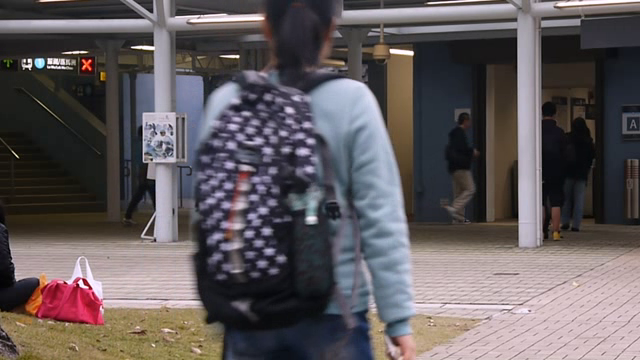
\includegraphics[width=\linewidth]{figures/qual/clip01_f965.png}
\end{minipage}\hfill
\begin{minipage}{0.47\linewidth}
  \centering\footnotesize
  \resizebox{\linewidth}{!}{%
  \begin{tabular}{@{}ll@{}}
  \toprule
  \multicolumn{2}{l}{\textbf{(a) clip 01, frame 965 (in GT)}}\\
  \midrule
  $r_{\text{pose}}$      & $0.781$ \\
  LOITERING strength     & $1.000$ \\
  belief $\mathrm{bel}(A)$ & $\mathbf{0.627}$ \\
  plausibility $\mathrm{pl}(A)$ & $0.944$ \\
  conflict $K$           & $0.100$ \\
  \bottomrule
  \end{tabular}}
\end{minipage}

\vspace{6pt}
% ---- (b) a benign scene that partially trips a cue, tempered by M1 -------
\begin{minipage}{0.45\linewidth}
  \centering
  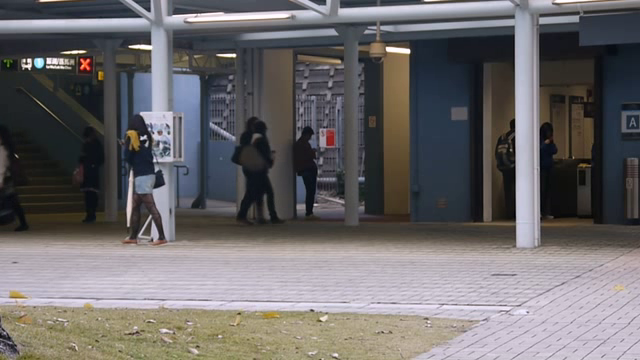
\includegraphics[width=\linewidth]{figures/qual/clip15_f939.png}
\end{minipage}\hfill
\begin{minipage}{0.47\linewidth}
  \centering\footnotesize
  \resizebox{\linewidth}{!}{%
  \begin{tabular}{@{}ll@{}}
  \toprule
  \multicolumn{2}{l}{\textbf{(b) clip 15, frame 939 (outside GT)}}\\
  \midrule
  $r_{\text{pose}}$      & $0.834$ \\
  LOITERING strength     & $1.000$ \\
  belief w/ M1           & $\mathbf{0.674}$ \\
  belief w/o M1 ($-$M1)  & $0.828$ \\
  conflict $K$           & $0.106$ \\
  \bottomrule
  \end{tabular}}
\end{minipage}
\caption{Two real evidence records from Avenue (raw fused belief
$\mathrm{bel}(A)$, pre-calibration). (a) A person standing still near a
stairwell with a large backpack for an extended dwell, inside a labeled
anomaly window: LOITERING fires at full strength and the fused belief
correctly clears $0.5$. (b) A person standing at an information board
outside any labeled anomaly window -- an everyday scene Avenue does not
call anomalous: LOITERING still fires (dwell time alone cannot distinguish
the two scenes), but a partially degraded skeleton ($r_{\text{pose}}=0.834$,
from viewing angle and partial occlusion) discounts the belief from $0.828$
(what the undiscounted, $-$M1 pipeline would output) to $0.674$ -- the
mechanism in \S\ref{sec:m1}--\S\ref{sec:m2} acting on a real frame, not a
synthetic one. Both frames carry non-trivial conflict $K\!\approx\!0.10$,
reflecting that LOITERING is the only cue active in either case.}
\label{fig:qual}
\end{figure}

\Cref{fig:qual} shows two real evidence records, both LOITERING-driven,
found by an exhaustive frame-level search of the Avenue test set (the
mechanism at work, not a cherry-picked illustration -- we searched every
frame of every one of the 21 test clips for the largest M1 effect and the
highest conflict, and report the winners). Panel (a) is a genuine alarm
inside a labeled anomaly window. Panel (b) is the clearest real case we
found of M1 tempering a cue on an ordinary scene Avenue does not label
anomalous: the same LOITERING cue fires at full strength as in panel (a),
but a partially degraded skeleton discounts the belief from $0.828$ (what
an undiscounted pipeline outputs on this exact frame) to $0.674$. We note
this frame does not fully cross to a suppressed alarm at the default
threshold -- an honest limit of what one still-active-cue example can show;
the aggregate effect of M1 across a whole stream is the controlled-noise
result in \S\ref{sec:m4} results ($19.2\to0.0$ FAPH), which is the claim
this section illustrates rather than replaces. In both frames LOITERING is
the sole active cue, so conflict $K$ stays modest ($\approx0.10$); we did
not find a frame with two disagreeing cues active simultaneously on the
Avenue test set, which is itself consistent with \Cref{tab:crossbench}'s
reading that Avenue's real anomalies mostly fall outside our five cues'
coverage.

% ==================================================================
\section{Limitations}
\label{sec:limits}

\emph{Reliability weighting is partly precedented.} The reliability-aware
prototype method \cite{reliabilityproto2026} weights one model's score by
keypoint confidence; our novelty is discounting
across a fused heterogeneous cue set with a conflict term and the downstream
calibration and guarantee, not the idea of using confidence.
\emph{Normal-stream hours.} M4 needs enough confirmed-normal video; several
pose-VAD benchmarks are short on it, so we report $\faph$ per available
normal-hour with intervals and mark budgets that cannot be certified.
\emph{Cue coverage.} The five cues target human-action anomalies; events such
as cycling or vehicle intrusion fall outside them, as for
\cite{yoloposeclip2026}. The fusion layer is cue-agnostic and could take on
additional cue types without redesigning M2--M4, but we have not built or
evaluated any.
\emph{Exchangeability.} Learn-then-Test assumes the calibration and deployment
normal streams are exchangeable; domain shift can break the guarantee, which
we treat as a measured outcome rather than an assumption.
\emph{Hardware.} Every latency number in this paper is measured on one
commodity laptop CPU (Intel Core i5-6300U); we have not measured on a
genuinely embedded-class device (e.g.\ a Jetson or Raspberry Pi), so the
decision layer's edge-deployability is currently evidenced on desktop-class
CPU only.
\emph{No operator study.} Part of this paper's motivation is that
uncalibrated alarms erode operator trust (\S\ref{sec:intro}); we have not run
a study with real operators to confirm that a calibrated probability and an
evidence record actually change trust or response behaviour in practice --
the outputs are designed for that purpose, but the effect is not yet
measured, on this system any more than on the prior work we compare against.
\emph{Real-data evidence for M1 is limited.} M1's one demonstrated benefit
(\S\ref{sec:m1ablation}) is a controlled result on a synthetic
corrupted-skeleton stream. On the four real datasets we checked for a
matching real-data effect, naturally low-reliability frames rarely coincide
with an active cue (under 25\% of active-cue frames, on every dataset and
cutoff we tried), and when they do it is almost always inside footage
already labelled anomalous rather than the confirmed-normal streams M1 is
meant to protect; the largest well-powered real subset we could isolate
(CHAD, low visible-joint-fraction frames with an active cue, $n{=}1355$)
shows no benefit ($\Delta\mathrm{AUC}=-0.041$). We report this rather than
let the synthetic result stand in for a real-data one it has not yet earned.
\emph{No threshold reaches $0.9$ event recall on any of the five benchmarks}
(\Cref{tab:crossbench}); the highest-recall FAPH cells are reported as
\emph{--} rather than filled in, so the false-alarms-per-hour claim in this
paper is demonstrated at the recall levels our sweep actually reaches, not
at the higher-recall operating point a deployment would likely prefer. We
checked whether this is an artifact of the threshold grid rather than the
data: sweeping down to the most permissive threshold possible (every frame
alarmed, not just our usual grid's floor of $\tau{=}0.02$) still only
recovers $16.7\%$ (Avenue), $45.1\%$ (NWPU-Campus), $48.3\%$
(ShanghaiTech), $68.8\%$ (CHAD) and $80.2\%$ (UBnormal) of ground-truth
events -- a real ceiling set by how many labelled anomalies our five cues
ever engage with at all, not a search-range limitation
(\texttt{calm/recall\_ceiling\_check.py}).
\emph{CALM-VAD's own detection accuracy does not exceed B0 by a meaningful
margin on any of the five benchmarks} (frame AUC delta $-0.005$ to $+0.003$,
\Cref{tab:crossbench} and per-dataset reports): the calibration and
risk-control gains in this paper are gains in what the fused belief means
and how its alarm rate is bounded, not in ranking quality, and should not be
read as evidence \method{} out-ranks a plain weighted sum.
\emph{Not a leaderboard result.} \method{} targets reliability and
deployability; it is not proposed as a new frame-AUC state of the art.

% ==================================================================
\section{Conclusion}

Deployable edge video anomaly detection fails at its back end, not its front
end: a black-box score and a hand-tuned threshold give operators neither a
usable probability, an auditable rationale, nor a bound on false alarms.
\method{} replaces that back end with four lightweight stages---front-end
reliability estimation, reliability-discounted evidence fusion, calibration,
and distribution-free alarm-rate control---and emits every alert as an
evidence record. Evaluated under a deployment-faithful protocol rather than
frame AUC on five real benchmarks, it produces a calibrated incident
probability with $56$--$95\%$ lower calibration error than the raw fused
belief on every one of them. A controlled study isolates the reliability
mechanism, removing false alarms caused by front-end degradation entirely
($19.2\to0.0$/h) without a detection cost. And given roughly an hour of
confirmed-normal calibration footage -- supplied deliberately on UBnormal or
found already sufficient in NWPU-Campus's own split -- it certifies an
operator-chosen alarm budget with a distribution-free guarantee on two
independent benchmarks, the first time this has been demonstrated for a
heuristic multi-cue video anomaly detector, all at a CPU cost of about
$0.1$--$1.5$\,ms per frame, independent of the dataset. Detection quality
itself is honestly uneven, tracking how much of each benchmark's anomaly
taxonomy the five underlying cues were built to see. We take the resulting
chance-level results on Avenue and NWPU-Campus -- reached for two different,
individually verified reasons -- as evidence the method is not overclaiming,
not as a failure to hide. The same two benchmarks are also where
cross-dataset calibration transfer is worst (\Cref{tab:cross}), a consistent
picture rather than an isolated result. Code and the evaluation harness are
released to make the protocol reusable, and to make the evaluation itself
complete: all $20$ cross-dataset pairs across all five benchmarks are
included.

% ==================================================================
\bibliographystyle{IEEEtran}
\bibliography{refs}

\end{document}
